LSPE-SWIPE (Short-Wavelength Instrument for the Polarization Explorer) 
is a mm-wave polarimeter aboard of a 
stratospheric balloon, aimed at measuring the polarization 
of the Cosmic Microwave Background at large angular scales. 
The general idea of SWIPE is to maximize the sensitivity to CMB 
polarization at large scales using a very wide focal plane populated 
with multi-moded bolometers. The spectral coverage of SWIPE has 
been optimized to be very sensitive to CMB polarization with one 
wide-band channel matching the peak of CMB brightness (140 GHz, 
33\% band), and to be able to monitor and separate the signals from 
interstellar dust (the main polarized foreground at this frequency) 
monitoring it with two ancillary channels at 220 and 240 GHz. These 
are narrow-band, (5\%) to measure the slope of the specific brightness 
of Interstellar dust. 
The focal planes of SWIPE are so large that 8800 modes of the 
incoming radiation are collected, thus boosting the sensitivity of the 
polarimeter to unprecedented levels. The detectors arrays are cooled 
at 0.3K by a large cryostat, which also cools the polarization modulator 
and the entire telescope. The cryostat is mounted in a frame (the gondola) 
providing also accommodation for an attitude control system, the 
instrument power system and electronics. The gondola interfaces 
to the flight train of the stratospheric balloon through an azimuth pivot 
allowing for azimuth scans and/or spin. 
A general view of the SWIPE instrument is shown in Figure~\ref{fig:swipe_overview}.
   \begin{figure}[h!]
   \centering
   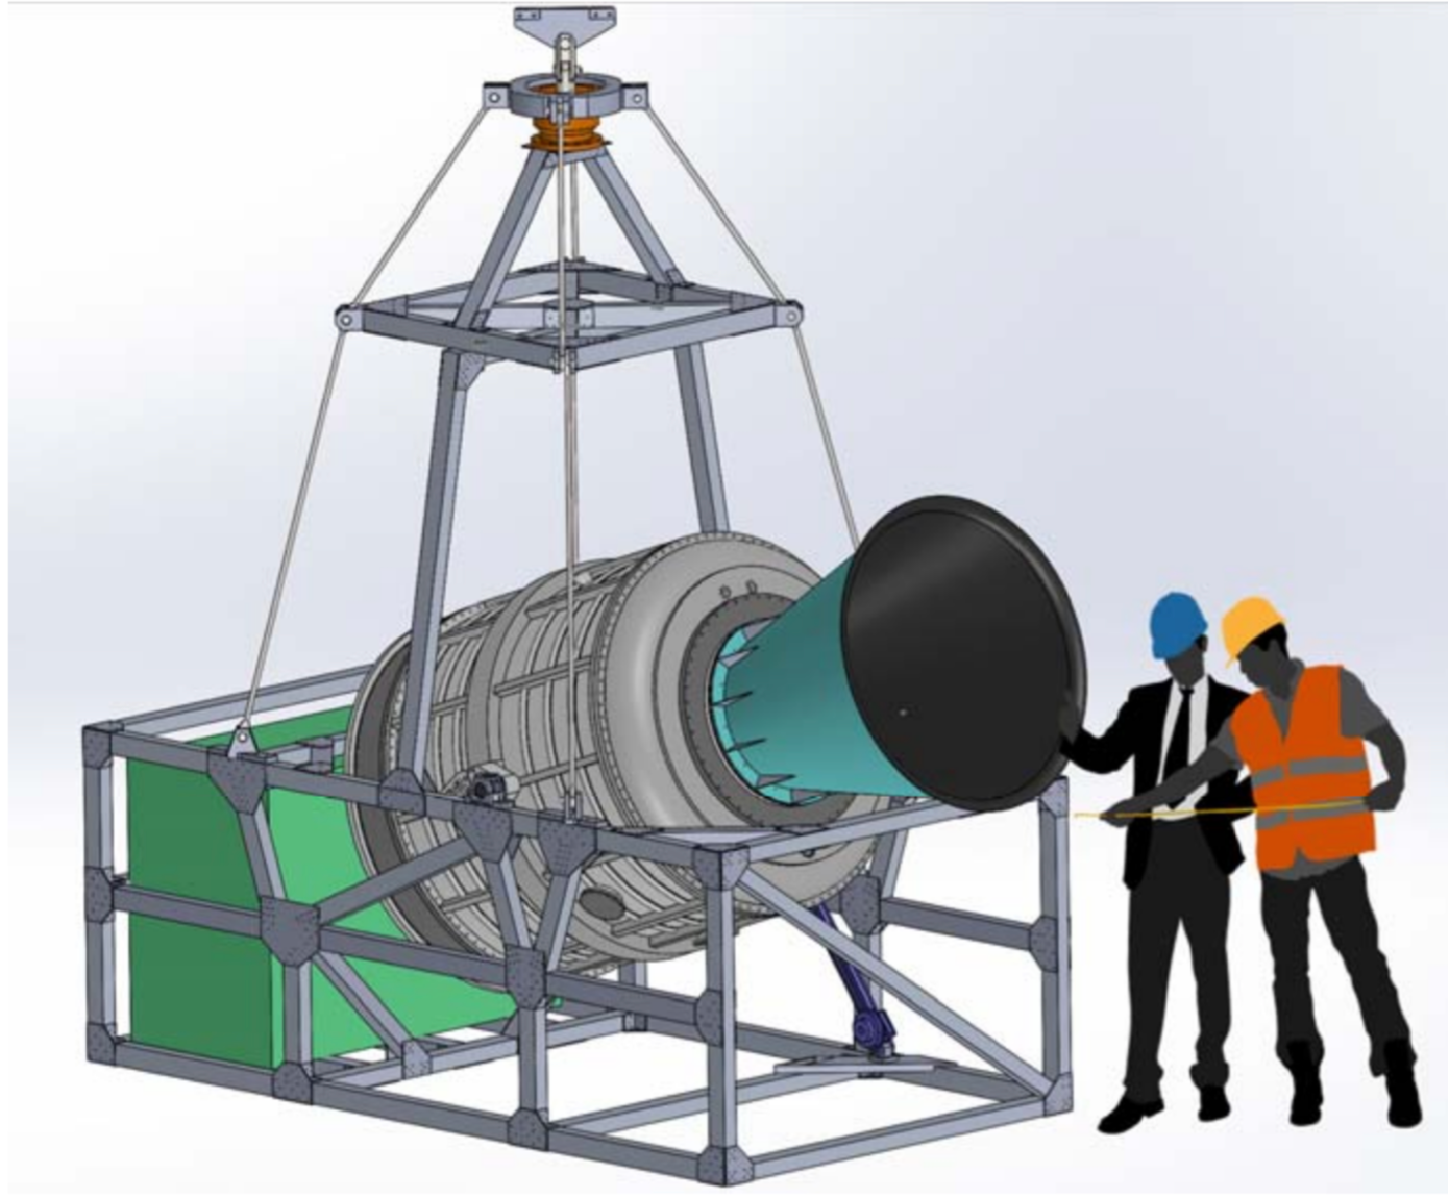
\includegraphics[width=8cm]{figs/swipe_overview.pdf}
   \caption{LSPE-SWIPE overview. The instrument is contained in a large 
   liquid Helium cryostat, which also contains the optical elements, including
   the HWP based Stokes polarimeter. The onboard electronics and the 
   Lithium batteries based power system are contained in an Aerogel 
   insulated box, to optimise thermal balance.  
  }
              \label{fig:swipe_overview}%
    \end{figure}

\subsubsection{Winter polar balloon flight}
\comment{Masi, Piacentini} \\
LSPE-SWIPE is designed to fly on a stratospheric long duration balloon in the arctic winter. 
Ballooning is needed to avoid most of the atmospheric emission, which is very relevant
at 140\,GHz and higher frequencies. The winter launch guarantees the possibility to 
cover a large sky fraction, thus exploring large angular scales of the CMB polarization. 
The instrument is designed to last 15 days. This long duration is needed to reach the
sensitivity to match the scientific goal od LSPE. 

Options for launching in the polar night are ate moment only possible from the 
northern hemisphere. In particular, two proposed launching station is 
Longyearbyen, in Spitsbergen island in Svalbard arcipelago (Norway), with a latitude 
above 78\,$^\circ$N; launches have been organised over the last years from 
this place, both in Summer and in Winter. 
As a more standard alternative, stratospheric balloon flights are organized by the Swedish 
Space Corporation in the Esrange Space Center, near Kiruna (Sweden), at
a latitude of 67.8\,$^\circ$N

Such a long duration flight in the Winter,
without solar illumination, is very demanding in terms of power system, and thermal 
balance. 
A series of technological test flights has been carried out over the years, as
reported in 
\citet{iarocci2008,peterzen_memsait2008,peterzen_cospar2008,peterzen_cospar2010,debernardisIAUS2013,wipica2018}.  
All the LSPE-SWIPE parts are designed to cope with temperatures as low as
$-90^\circ$C, except the battery pack and part of the electronics which is contained in 
a thermally insulated box, designed to work above $-40^\circ$C. This box is insulated
by means of Aerogel. A prototype of this power system was flown in a winter Arctic balloon 
in December 2017 \citep{wipica2018}. 


\subsubsection{Optical system}
\comment{de Bernardis, Lamagna} \\
The optical system of LSPE-SWIPE (Figure~\ref{fig:swipe_optics}) consists in a single-lens, 
490\,mm aperture refractor telescope, focusing incoming radiation 
on two large curved focal planes, split by a large wire-grid polarizer. 
Each focal plane is populated with 165 multi-moded feed-horns, 
each feeding a spider-web Transition Edge Superconducting (TES) 
bolometer. Polarization modulation is obtained rotating a large 
half-wave-plate (HWP) which is the first optical element of the optical 
system.
   \begin{figure}[h!]
   \centering
   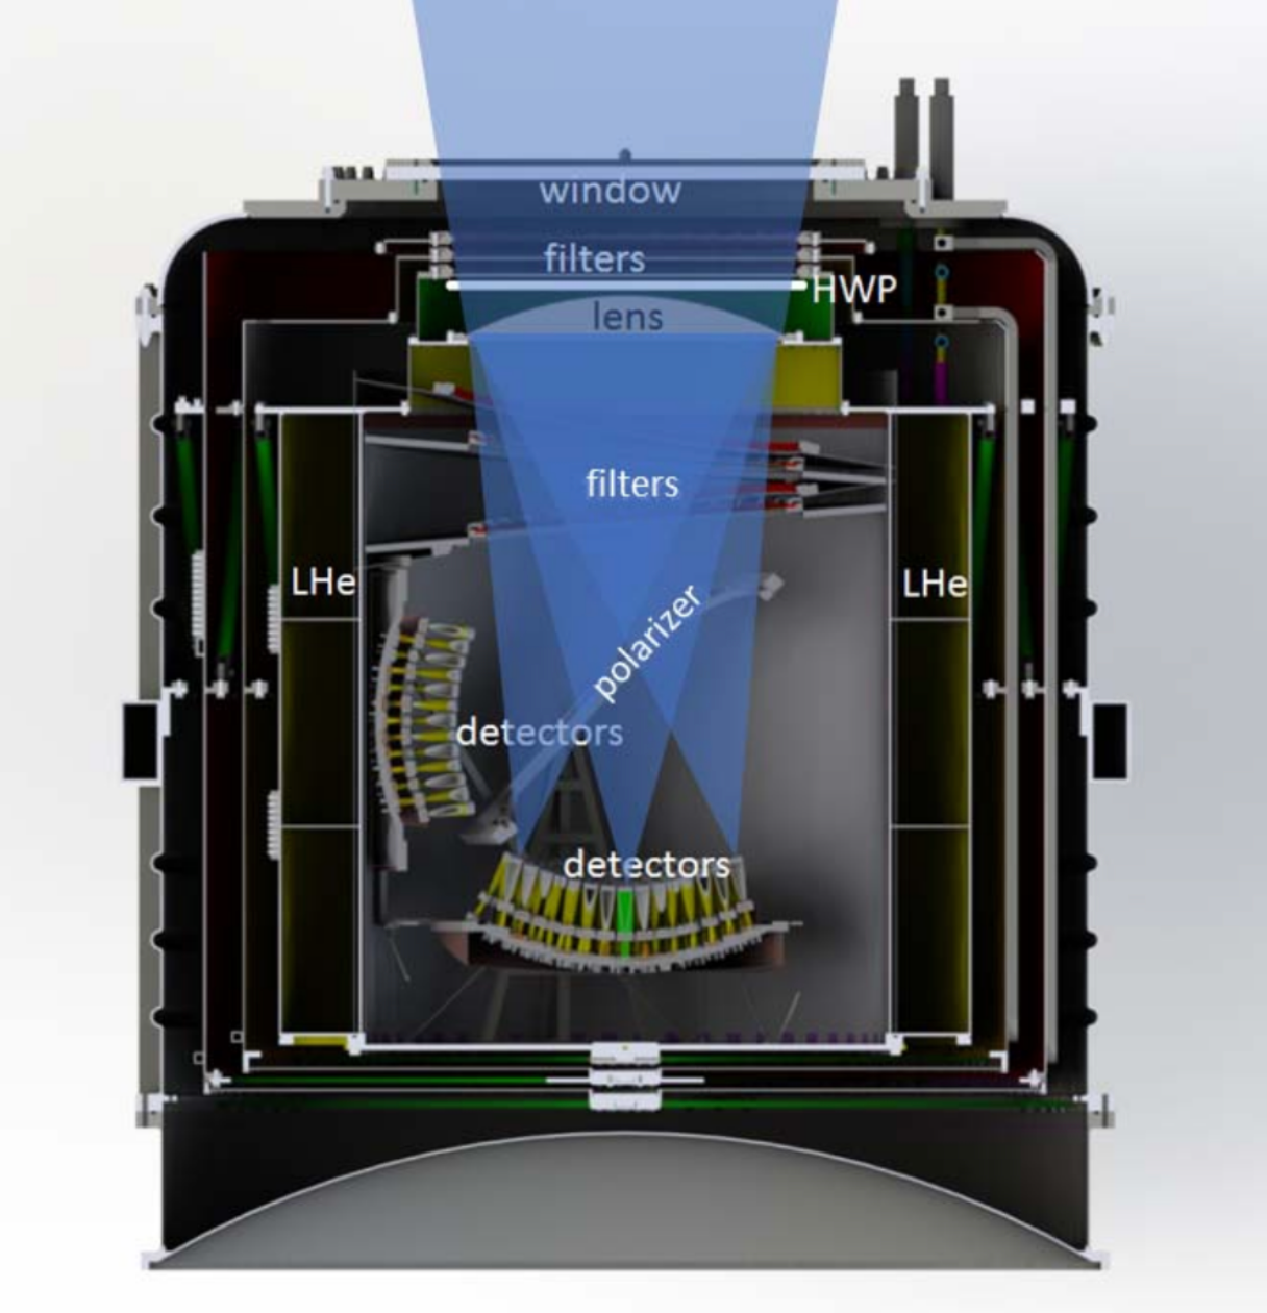
\includegraphics[width=8cm]{figs/swipe_optics_3d}
   \caption{LSPE-SWIPE cryostat and optical optical system
   \comment{Need better figure}}
              \label{fig:swipe_optics}%
    \end{figure}
    
The configuration fulfils our requirements with a low cross-polarization (<0.2\%) 
and a controlled instrumental polarization (an absorption polarization <0.2\% 
and an emitted component reduced and stable by the use of a cold telescope). 
These goals are reached at the edge of the corrected focal plane for all the 3 
bands and they are totally negligible on axis. 
Besides the 490\,mm in diameter lens the optics is completed by a 460\,mm in 
diameter cold stop close to the lens (corresponding to an entrance pupil of 
487\,mm in diameter). 
The FOV, 20\,degrees wide, is split by a 500\,mm in diameter 45\,degress tilted wire grid 
in 2 curved focal plane (CFP\_T and \_R) 300\,mm in diameter both with 
a f/number equal to f/1.75.
The full optical system is kept at cryogenic temperature into the LSPE-SWIPE cryostat, 
in order to minimize radiative background and variable emission from the 
rotating HWP. 

The radiation is coupled to the detectors by means of multimode horns
\citep{legg2016} ....

\comment{Lamagna: add details on horns, in particular mode-coupling}

\subsubsection{Polarization modulation}
\comment{Pisano, Columbro, de Bernardis} \\
In order to modulate the polarized component of the signal, LSPE-SWIPE adopts 
Stokes polarimeter based on a Half Wave Plate (HWP) built of metal mesh 
metamaterials. This technology has been developed by the Instrumentation Group 
at the Department of Physics and Astronomy of the Cardiff University, and 
guarantees homogenous performance over a wide range of frequencies. 

\comment{Pisano: add details about HWP performance}



\subsubsection{Detectors}

\comment{sempre nell'ottica di definire le prestazioni, quindi modi accoppiati, efficienza, 
time constants, e noise}
\\ \comment{Gatti / Lamagna}



